\documentclass[xcolor=dvipsnames, compress]{beamer}
%\usetheme{Madrid} % My favorite!
\usetheme{Boadilla} % Pretty neat, soft color.
%\usetheme{Warsaw}
%\usecolortheme{dove} 
%\usetheme[secheader]{Boadilla}
% \useoutertheme[subsection=false]{smoothbars}
% \useinnertheme{rectangles}
% \usetheme{Marburg}
%   \usecolortheme[RGB={139,10,80}]{structure}
%  \usecolortheme[RGB={25,25,112}]{structure}
%\usecolortheme[RGB={255,127,36}]{structure}
%\usetheme{CambridgeUS}
%\usetheme{PaloAlto}
% \usefonttheme{professionalfonts}
% \usepackage{listings}

\usetheme{Boadilla}

% \usetheme{Warsaw}
%\usetheme{Darmstadt} %OK!
%  \usetheme{Frankfurt} %OK!
% \usetheme{Goettingen}
% \usetheme{Dresden}
%\usetheme{JuanLesPins} %OK!!
%\usetheme{Marburg}
%  \usetheme{Montpellier}
% \usetheme{Rochester} %sobrio
%\usetheme{Singapore}
%\usetheme{Szeged}
%\usetheme{Luebeck}

%\usetheme{Hannover}
%\usecolortheme{wolverine}

%\usecolortheme{albatross}
%\usecolortheme{seahorse}
%\usecolortheme{beetle}
%\usecolortheme{crane}
%\usecolortheme{dolphin}
%\usecolortheme{dove} %<- este con orchid
%\usecolortheme{fly}
%\usecolortheme{lily}
%\usecolortheme{orchid}
%\usecolortheme{rose}
%\usecolortheme{seagull}
%\usecolortheme{whale}

%\usetheme{Bergen} % This template has nagivation on the left
%\usetheme{Frankfurt} % Similar to the default 
%with an extra region at the top.
%\usecolortheme{seahorse} % Simple and clean template
%\usetheme{Darmstadt} % not so good
% Uncomment the following line if you want %
% page numbers and using Warsaw theme%
% \setbeamertemplate{footline}[page number]
%\setbeamercovered{transparent}
%\setbeamercovered{invisible}
% To remove the navigation symbols from 
% the bottom of slides%
%\setbeamertemplate{navigation symbols}{} 
%
\usepackage{graphicx}
\usepackage{amssymb,amsmath,amscd}
\usepackage{latexsym,xspace}
\usepackage[utf8]{inputenc}
\usepackage{epsfig}
%\usepackage{fancyhdr}
%\usepackage[spanish]{babel}
\usepackage[all]{xy}
\usepackage{enumerate}
\usepackage{eucal}
%\usepackage[usenames]{color}

\usepackage{mathtools} % flechas con nombres arriba o abajo


%#########################
\newcommand{\tx}{\ensuremath{\tau(X)}}
\newcommand{\txx}{\ensuremath{\tau_{X}}}
\newcommand{\Q}{\ensuremath{\mathbb{Q}}}
\newcommand{\Z}{\ensuremath{\mathbb{Z}}}
\newcommand{\N}{\ensuremath{\mathbb{N}}}
\newcommand{\R}{\ensuremath{\mathbb{R}}}
\newcommand{\C}{\ensuremath{\mathbb{C}}}
\newcommand{\A}{\ensuremath{\forall}}
\newcommand{\E}{\ensuremath{\exists}}
\newcommand{\iso}{\ensuremath{\cong}}
\newcommand{\union}{\ensuremath{\cup}}
%\newcommand{\morinyec}{\ensuremath{\precapprox}}
%\newenvironment{prueba}{\vspace{-3mm}\noindent\textbf{Demostraci\'on}\\}{\noindent$\blacksquare$\\}
\newcommand{\nin}{\ensuremath{\notin}}
\renewcommand{\emptyset}{\varnothing}

%\newcommand{\niso}{\ensuremath{\not \cong}}
\newtheorem{teor}{Teorema}[section]
\newtheorem{defi}{Definition}[section]
\newtheorem{ejemplo}{Examples}[section]
\newtheorem{obs}{Remark}[section]
\newtheorem{prop}{Proposition}[section]
\newtheorem{cor}{Corollary}[section]
\newtheorem{ntc}{Notation}[section]
\newtheorem{lema}{Lemma}[section]
\newtheorem{prob}{Problem}
\newtheorem{comen}{Comment}

%\usepackage{bm}         % For typesetting bold math (not \mathbold)
%\logo{\includegraphics[height=0.6cm]{yourlogo.eps}}
%
\title[Hidden Markov Chains]{Hidden Markov Chains}
\author{Marco, Nicolás, Sebastián \& César}
\institute[ITAM]
%\date{November 7, 2019}
% \today will show current date. 
% Alternatively, you can specify a date.
%


\begin{document}
%
\begin{frame}
\titlepage
\end{frame}

\begin{frame}
\frametitle{Index}
 \tableofcontents%[sections]
\end{frame}


\begin{frame}
\section{Motivation }
\frametitle{Reminder: What a Markov chain is?}
\begin{itemize}	
	\item A Markov chain is a stochastic process with a particular characteristic, must be "memory-less" (i.e the probability of future actions are not dependent upon the steps that led up to the present state.). This property is known as the \textbf{Markov property}.
	\item We can find very often phenomena that satisfy the Markov property. This fact make Markov chains very useful in various application scenarios.
	\item Additionally, Markov chains allow us modeling sequential processes in a simple but effective way.	
\end{itemize}
\end{frame}

\begin{frame}
\section{Markov chains}
\frametitle{Reminder: What a Markov chain is?}
A simple example...
\begin{itemize}
\item Bag of balls without replacement: \textbf{is NOT} a Markov process
\begin{figure}
	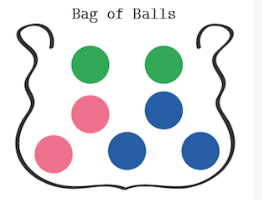
\includegraphics[scale=0.25]{images/ex1_bag_of_balls.png}
	\caption{example: probability of getting a blue ball / without replacement}
\end{figure}
\item Bag of balls with replacement \textbf{is} a Markov process
\begin{figure}
	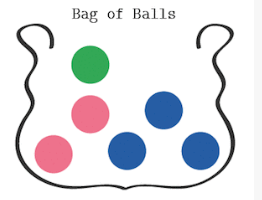
\includegraphics[scale=0.25]{images/ex1_bag_of_balls_wrep.png}
	\caption{example: probability of getting a blue ball / with replacement}
\end{figure}
\end{itemize}
\end{frame}
%

\begin{frame}
\frametitle{Markov chains: Definition}

\begin{block}{Markov Chain: definition}
	A Markov chain is a sequence $X_{0:T}=\left(X_{0},X_{1},\ldots,X_{T}\right)$  of random variables taking values in some finite set $\mathcal{X}$ that satisfies the rule of conditional independence:
	\begin{equation*}
	{P}\left(X_{t+1}=x_{t+1}\mid X_{t}=x_{t},\ldots,X_{0}=x_{0}\right)= {P}\left(X_{t+1}=x_{t+1}\mid X_{t}=x_{t}\right)
	\end{equation*}	
\end{block}

For this case, we will study time-homogeneous Markov chains (i.e. the probability of any state transition is independent of time).\begin{equation*}
A_{i,j}:={P}\left(X_{t+1}=j\mid X_{t}=i\right)\:i,j\in\mathcal{X}
\end{equation*}

However, the general case of Markov chains allows for time-inhomogeneous Markov chains (as time goes on, the probability of moving from one state to another may change). 

\end{frame}


\begin{frame}
\frametitle{Transition matrices}
Movements among states are defined by a \textbf{transition matrix}, $A_{t}$. which contains information on the probability of transitioning between states. 
\begin{equation*}
A_{i,j}:={P}\left(X_{t+1}=j\mid X_{t}=i\right)\:i,j\in\mathcal{X}
\end{equation*}		
Each row of the matrix is a probability vector, with sum of its entries is 1. 

Given $x_{0}\in\mathcal{X}$, let $\mu_{x0}={P}\left(X_{0}=x_{0}\right)$; joint probability mass function of $X_{1:T}$ in terms of $\left(A_{i,j}\right)_{i,j\in\mathcal{X}}$ and $\left(\mu_{i}\right)_{i\in\mathcal{X}}$ is:
\begin{eqnarray*}
p\left(x_{0:T}\right) & := & {P}\left(X_{0}=x_{0},\ldots,X_{T}=x_{t}\right)\\
& =& {P}\left(X_{0}=x_{0}\right)\prod_{t=1}^{T}{P}\left(X_{t}=x_{t}\mid X_{t-1}=x_{t-1}\right)\\
& = & \mu_{x0}\prod_{t=1}^{T}A_{x_{t-1},x_{t}}
\end{eqnarray*}		
\end{frame}
%
\begin{frame}
\section{Hidden Markov Chains }
\frametitle{Hidden Markov Chains : Motivation}
\begin{itemize}
\item A  \textbf{Hidden Markov Model} is a statistical model which studies a system assumed as a Markov process including hidden (unobservable) states. 
\item In the simple Markov chain model, the state of the system is directly visible to the observer. 
\item On the other hand, HMM assume that the data observed is not the actual state of the model but instead is generated by underlying hidden states.
\item Each state has a probability distribution over the possible outputs. 
\item HMM are often used to model temporal data.
\end{itemize}
\end{frame}
%
\begin{frame}
\frametitle{Definition}
\begin{block}{HMM :Definition}
Let $X_{0:T}=\left(X_{0},X_{1},\ldots,X_{T}\right)$ be a homogeneous Markov chain taking values in $\mathcal{X}$ with and associated transition matrix $\left(A_{ij}\right)$. Additionally, there exits another sequence of random variables $Y_{0:T}=\left(Y_{1},\ldots,Y_{T}\right)$ taking values in $\mathcal{Y}$, known as the observation space. 
\end{block}	

We assume that the random variables of sequence $Y_{0:T}$ are independent conditional on the state sequence $X_{0:T}$, which is equivalent to:
\end{frame}

\begin{frame}
\begin{equation*}
{P}\left(Y_{1}=y_{1},\ldots,Y_{T}=y_{T}\mid X_{0}=x_{0},\ldots,X_{T}=x_{t}\right)
\end{equation*}	
\begin{equation*}
=\prod_{t=1}^{T}{P}\left(Y_{t}=y_{t}\mid X_{t}=x_{t}\right)
\end{equation*}	

if we are considering an homogeneous HMM, then we have an  \textbf{emission probability} mass function:
\begin{equation*}
g_{x}(y):={P}\left(Y_{t}=y\mid X_{t}=x\right)
\end{equation*}	
\end{frame}
%
\begin{frame}
\frametitle{More Definitions}
Using the emission probabilities to connect the observation space and the hidden space and introducing the transition matrix that governs the movements among hidden states, we can define the  joint probability of the hidden states and observations as follows:
\begin{equation*}
{P}\left(X_{0:T}=x_{0:T},Y_{0:T}=y_{0:T}\right)=\mu_{x_{0}}\prod_{t=1}^{T}g_{x_{t}}\left(y_{t}\right)A_{x_{t-1},x_{t}}
\end{equation*}	
\end{frame}

%%%%%%%%%%%%%%%%%%%%

\begin{frame}
\frametitle{Inference in Hidden Markov Models (HMM)}
\begin{block}{Remark:}
For simplicity of exposure \textbf{we consider discrete-valued observations} $Y_t$, however algorithms apply similarly with continuous observation.
\end{block}
\vspace{0.3cm}

\textbf{Some notations:}
\begin{itemize}
	\item $p(x_{t+1}|x_t) = P( X_{t+1}= x_{t+1}|X_t = x_t)$
	\item $p(y_{t}|x_t) = P( Y_{t}= y_{t}|X_t = x_t)$
	\item $p(x_{t}|y_{1:t}) = P( X_{t}= x_{t}|Y_1 = y_1, \ldots, Y_t = y_t )$
	\item $p(y_{1:t}) = P(Y_1 = y_1, \ldots, Y_t = y_t )$
\end{itemize}
\end{frame}

\begin{frame}
\frametitle{What do you mean by inference problems in HMM?}
 \textbf{Filtering:}\\
  Given measurements up to time $t$, compute the distribution of $X_t$, $$p(x_{t}|y_{1:t})$$
\begin{center}
	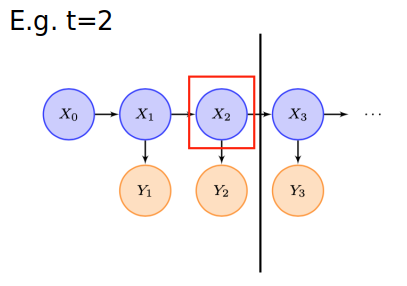
\includegraphics[width=0.45\textwidth]{images/m_filtering.png}
\end{center}
\end{frame}

\begin{frame}
\frametitle{What do you mean by inference problems in HMM?}
\textbf{Prediction:}\\ Given measurements up to time $\textcolor{red}{s<t}$, compute the distribution of $X_t$, $$p(x_{t}|y_{1:s})$$ 
\begin{center}
	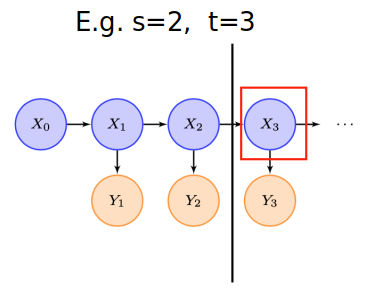
\includegraphics[width=0.45\textwidth]{images/m_smooth.png}
\end{center}

\end{frame}

\begin{frame}
\frametitle{What do you mean by inference problems in HMM?}
 \textbf{Smoothing:}\\ Given measurements up to time $\textcolor{red}{s>t}$, compute the distribution of $X_t$, $p(x_{t}|y_{1:s})$.
\begin{center}
	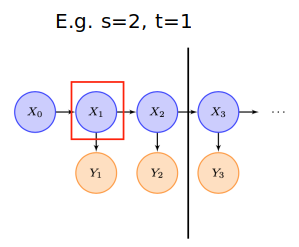
\includegraphics[width=0.4\textwidth]{images/m_smooth2.png}
\end{center}

\end{frame}

\begin{frame}
\frametitle{What do you mean by inference problems in HMM?}
 \textbf{Likelihood:}\\ Given observations $y_1, \ldots, y_T$ compute its likelyhood model,  $$p(y_{1:T})$$
\begin{center}
	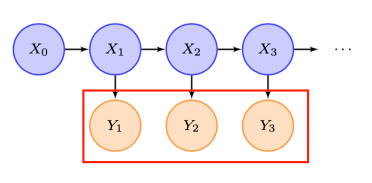
\includegraphics[width=0.6\textwidth]{images/m_likelihood.png}
\end{center}
\end{frame}

\begin{frame}
\frametitle{What do you mean by inference problems in HMM?}

\begin{columns}
	\begin{column}{0.5\textwidth}  %%<--- here
	\textbf{Decoding:}\\ Find the most likely state history $\mathcal{X}$ given the observation history: $$arg \max_{x_{0:t}} p(x_{0:T} | y_{1:T})$$		
	\end{column}
	\begin{column}{0.5\textwidth}
	\begin{center}
		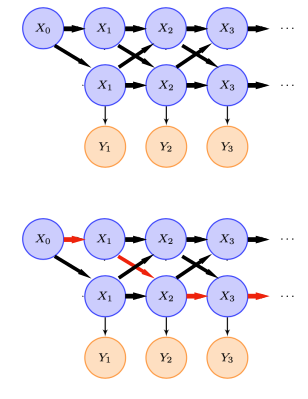
\includegraphics[width=0.7\textwidth]{images/m_decoding.png}
	\end{center}
	
\end{column}
\end{columns}
\end{frame}

\begin{frame}
\frametitle{Example: Hidden Mark-frog Chains}
\begin{center}
	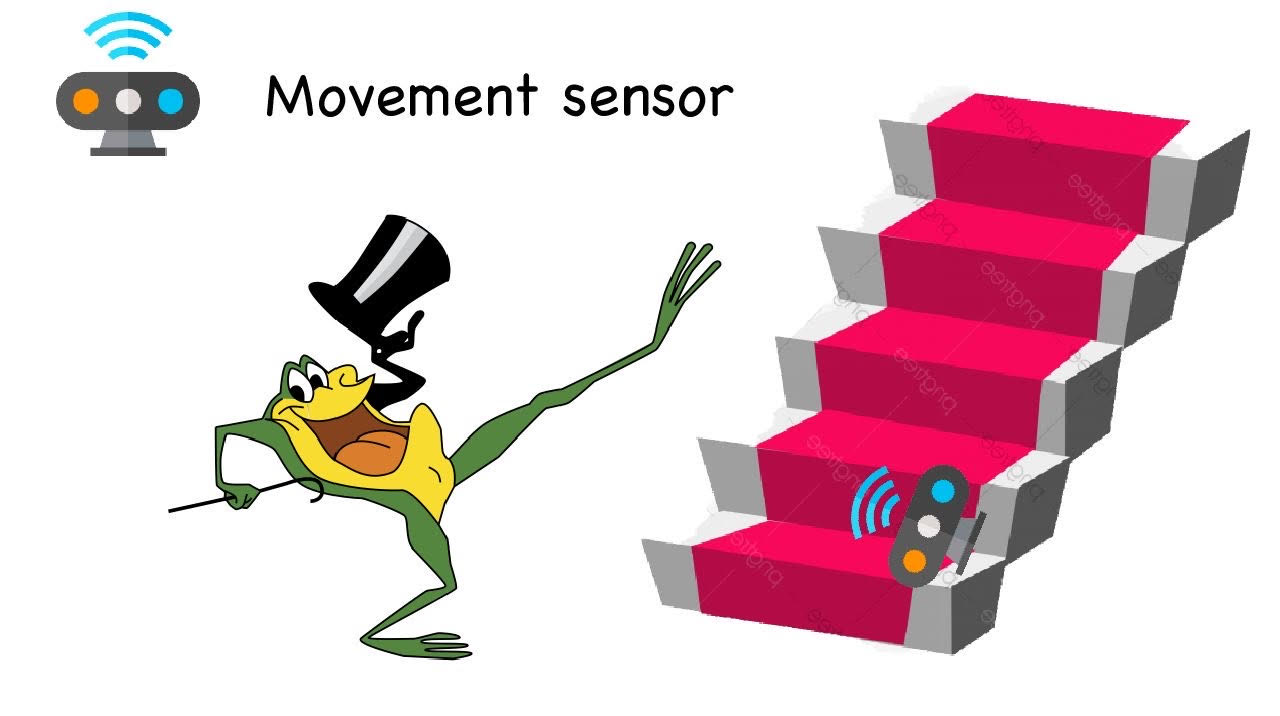
\includegraphics[width=1.0\textwidth]{images/frog_ladder.jpg}
\end{center}

\end{frame}


\begin{frame}

\begin{columns}
\begin{column}{0.3\textwidth}
	\begin{center}
		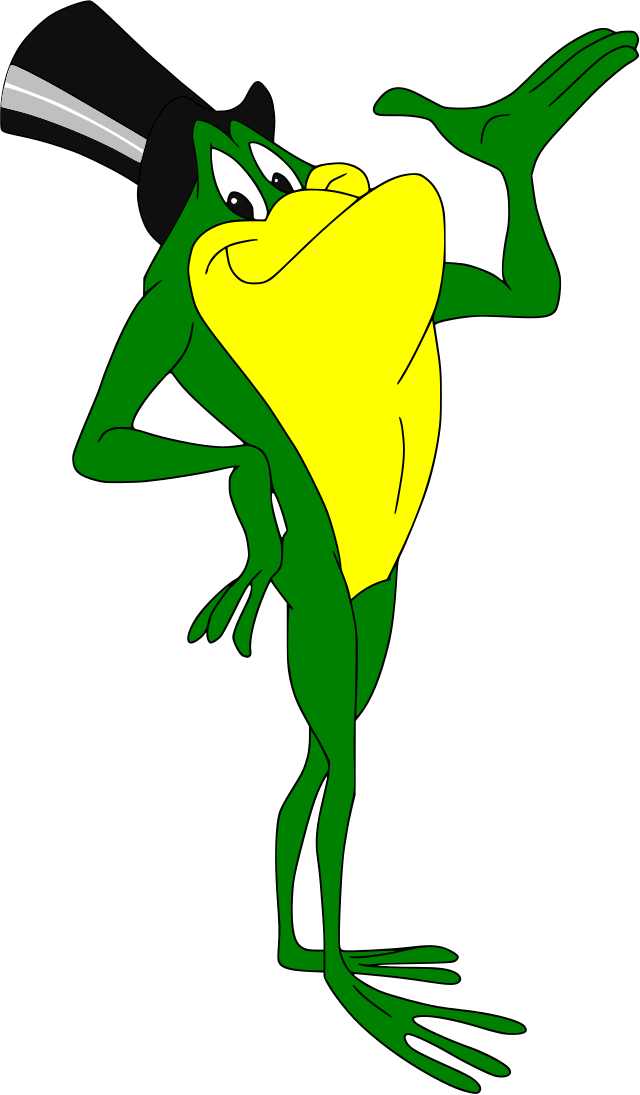
\includegraphics[width=0.7\textwidth]{images/frog2.png}
	\end{center}
	
\end{column}
\begin{column}{0.6\textwidth}  %%<--- here
	
	\begin{itemize}
		\item Our frog is jumping on a ladder with $K=6$ levels.
		\item From position $X_t$ level at which the frog is at time $t$ is \textbf{not observed}.
		\item Frog’s detector at the lowest level of the ladder sends a signal$Y_t$ $$Y_t=1 \mbox{ }non-detection$$ $$Y_t=2 \mbox{ }detection$$
		\item Observations $$y_{1:14} = (1, 1, 1, 1, 2, 2, 1, 1, 1, 1, 2, 2, 1, 2)$$
	\end{itemize}		
	
\end{column}
\end{columns}
\end{frame}

\begin{frame}
\begin{columns}
\begin{column}{0.5\textwidth}
\textbf{Transition matrix}
$p=0.4$
$$A_{1,2} = 1-p, A_{K,1} = \frac{1-p}{2}$$
$$ A_{i,i+1} = \frac{1-p}{2} \mbox{ for } i=1,\ldots, K-1$$
$$ A_{i,i} = p \mbox{ for } i=1,\ldots, K$$
$$ A_{i,i-1} = \frac{1-p}{2} \mbox{ for } i=2,\ldots, K$$
\end{column}
\begin{column}{0.5\textwidth}  %%<--- here
\textbf{Probability of detection}
$$B_{k,2}:= P(Y_t=2|X_t=k) $$ 
$$=\begin{cases} 0.9 &\mbox{if } k=1 \\
0.5 & \mbox{if } k=1 \\
0.1 & \mbox{if } k=2 \\
0 & \mbox{ } otherwise
\end{cases}$$	

\end{column}
\end{columns}

\vspace{0.5cm}

\textbf{Problems:} From frog’s observations of position at each time $t$, infer 1) filtering and 2) smoothing and 3) MAP estimate of pmf's.

\end{frame}

%
%% Marco Diap 12
\begin{frame}
\frametitle{Where can the frog jump? - Transition probabilities (Matrix A)}

\begin{center}
\begin{table}
\begin{centering}
\textbf{Level to}
\par\end{centering}
\begin{centering}
\textbf{Level from}
\begin{tabular}{|c|c|c|c|c|c|c|}
\hline 
%\rowcolor{lightgray}
& 1 & 2 & 3 & 4 & 5 & 6\tabularnewline
\hline 
\hline 
1 & 0.4 & 0.6 &  &  &  & \tabularnewline
\hline 
2 & 0.3 & 0.4 & 0.3 &  &  & \tabularnewline
\hline 
3 &  & 0.3 & 0.4 & 0.3 &  & \tabularnewline
\hline 
4 &  &  & 0.3 & 0.4 & 0.3 & \tabularnewline
\hline 
5 &  &  &  & 0.3 & 0.4 & 0.3\tabularnewline
\hline 
6 & 0.3 &  &  &  & 0.3 & 0.4\tabularnewline
\hline 
\end{tabular}
\par\end{centering}
\caption{Hidden Mark-frog chain example - Part I}

\end{table}
\par\end{center}
\end{frame}
%

%% Marco Diap 11
\begin{frame}
\frametitle{Where is the frog at the beginning?}

%\begin{center}

\begin{table}
	\begin{centering}
		\begin{tabular}{|c|c|c|c|c|c|}
			\hline 
			1 & 2 & 3 & 4 & 5 & 6\\
			\hline 
			\hline 
			1/6 & 1/6 & 1/6 & 1/6 & 1/6 & 1/6\\
			\hline 
		\end{tabular}
	\end{centering}
	\caption{Hidden Mark-frog chain example - Part II}
\end{table}
%\par\end{center}
\end{frame}

%% Marco diap 13
\begin{frame}
\frametitle{What is the probability of detecting the frog? - Emission probabilities (Matrix B)}

\begin{center}
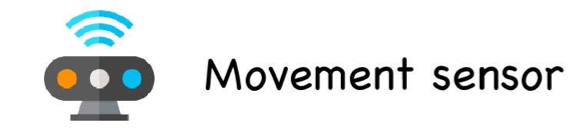
\includegraphics[width=0.4\textwidth]{images/sensor.png}
\end{center}

\begin{center}
	\textbf{At Level k, probabilitiy of being:}
\end{center}

\begin{center}
\begin{table}
\begin{centering}
\begin{tabular}{|c|c|c|}
\hline 
At Level & Detected & Not detected\tabularnewline
\hline 
\hline 
1 & 0.9 & 0.1\tabularnewline
\hline 
2 & 0.5 & 0.5\tabularnewline
\hline 
3 & 0.1 & 0.9\tabularnewline
\hline 
4 & 0 & 1\tabularnewline
\hline 
5 & 0 & 1\tabularnewline
\hline 
6 & 0 & 1\tabularnewline
\hline 
\end{tabular}
\par\end{centering}
\caption{Hidden Mark-frog chain example - Part III}
\end{table}
\par\end{center}
\end{frame}
%
%% Marco diap 14
%\begin{frame}
%\frametitle{Example - Observations}
%After 14 times, this are the sensor\textquoteright s results: 
%\begin{center}
%\begin{table}
%\begin{centering}
%\begin{tabular}{|c|c|c|c|c|c|c|c|c|c|c|c|c|c|}
%\hline 
%1 & 2 & 3 & 4 & 5 & 6 & 7 & 8 & 9 & 10 & 11 & 12 & 13 & 14\tabularnewline
%\hline 
%\hline 
%0 & 0 & 0 & 0 & 1 & 1 & 0 & 0 & 0 & 0 & 1 & 1 & 0 & 1\tabularnewline
%\hline 
%\end{tabular}
%\par\end{centering}
%\caption{Hidden Mark-frog chain example - Part IV}
%\end{table}
%\par\end{center}
%\end{frame}
%
%% Marco diap 15
\begin{frame}
\frametitle{Filtering (using Forward algorithm)}
\textbf{Forward Algorithm initialization equation}
$$ \alpha_{1}(i) = \pi_i \cdot b_{i}(O) $$

\textbf{Forward Algorithm recursion equation}
$$ \alpha_{t+1}(j) = \sum_{i=1}^N \alpha_t(i) \alpha_{ij} b_{ij}(O) $$

\textbf{Termination}
$$ P(O|\lambda) = \sum_{i=1}^N \alpha_T(i)$$
\end{frame}
%

%% Marco diap 19 (las imagenes de sus diap 16, 17 y 18 se movieron mas adelante)
\begin{frame}
\frametitle{Formal Filtering}
We are interested in the conditional probability mass function $p\left(x_{t}\mid y_{1:t}\right)$ of the state $X_{t}$ given the data observed up to time $t$ .

$$ p(x_t|y_{1:t}) = \frac{p(x_t, y_{1:t})}{ \sum_{x_t^\prime \in \mathcal{X}} p(x_t^\prime, y_{1:t}) }$$

\end{frame}
%
\begin{frame}
\frametitle{Formal Filtering}
We will derive a recursion for:
\hspace{-0.2cm}
\begin{eqnarray*}
\textcolor{red}{p(x_t,y_{t	:T})} & = & \sum_{x_{t-1} \in \mathcal{X}} p(x_t, x_{t-1}, y_t, y_{1:t-1})\\
& = & \sum_{x_t \in \mathcal{X}} p(y_{t}| x_t, x_{t-1}, y_{1:t-1} ) p(x_{t} |x_{t-1},y_{1:t-1}) p(x_{t-1},y_{1:t-1}) \\
& = &  p(y_{t}|x_t) \sum_{x_t \in \mathcal{X}} p(x_{t}|x_{t-1}) \textcolor{red}{ p(x_{t-1},y_{1:t-1})}   
\end{eqnarray*}

If we define $\alpha(t):= p(x_{t},y_{1:t})$, then we have a forward recursion for $t=1, \ldots, T$, $x_t\in \mathcal{X}$:
$$ \textcolor{red}{\alpha_{t}(x_{t})} = p(y_{t}|x_t) \sum_{x_t \in \mathcal{X}} p(x_{t}|x_{t-1}) \textcolor{red}{\alpha_{t-1}(x_{t-1})}; \mbox{ } \alpha_0(x_0)=0 $$
\end{frame}
%
%% Marco diap 20
\begin{frame}
\frametitle{Formal Filtering and likelihood}
So, we compute a filtering using: 

For $t=1,\ldots,T$, $x\in X$:

\[
\alpha_{t}\left(x_{t}\right)=p\left(y_{t}\mid x_{t}\right)\sum_{x_{t-1}\in\mathcal{{X}}}p\left(x_{t}\mid x_{t-1}\right)\alpha_{t-1}\left(x_{t-1}\right)
\]	

The filtering pmf is obtained by normalizing $\alpha_{t}\left(x_{t}\right)$
as: 
$$p(x_t| y_{1:t}) = \frac{p(x_t, y_{1:t})}{p(y_{1:t})}  = \frac{\alpha_t(x_t)}{ \sum_{x \in \mathcal{X}} \alpha_t(x) }$$
\end{frame}
%
\begin{frame}
\frametitle{Formal Filtering and likelihood}


The likelihood term $p\left(y_{1:t-1}\right)$ can be computed from
the $\alpha$-recursion:
$$p(y_{1:T}) =  \sum_{x \in \mathcal{X}} \alpha_T(x) $$

\end{frame}
%
%% Marco diap 21
\begin{frame}
\frametitle{Considerations in Filtering}
\begin{itemize}
\item  Proposed recursion may suffer from numerical stability (underflow, overflow),
as $\alpha_{t}$ may become very small or very large for large $t$. 
\item To avoid this, we can normalize $\alpha_{t}$, or propagate the filtering
\emph{pmf $p\left(x_{t}\mid y_{1:t}\right)$ }instead of $\alpha_{t}$,
using the following two-step predict-update recursion:
\end{itemize}
$$
p\left(x_{t}\mid y_{1:t-1}\right)=\sum_{x_{t-1}\in\mathcal{{X}}}p\left(x_{t}\mid x_{t-1}\right)p\left(x_{t-1}\mid y_{1:t-1}\right)\qquad Predict
$$

$$
p\left(x_{t}\mid y_{1:t}\right)=\frac{g_{x_{t}}\left(y_{t}\right)p\left(x_{t}\mid y_{1:t-1}\right)}{\sum_{x_{t}^{'}\in\mathcal{{X}}}g_{x'_{t}}\left(y_{t}\right)p\left(x'_{t}\mid y_{1:t-1}\right)}\qquad Update
$$
\end{frame}

\begin{frame}
\frametitle{Example: Hidden Mark-frog Chains - Filtering pmf}
\begin{center}
	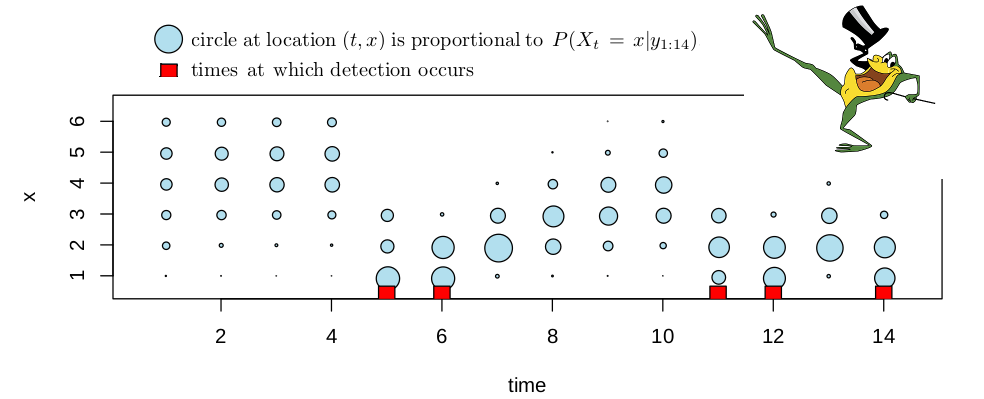
\includegraphics[width=1.01\textwidth]{images/frog_filtering.png}
\end{center}
\end{frame}

\begin{frame}
\section{Smoothing}
\frametitle{Smoothing}

\textbf{General problem of smoothing:}\\
\textbf{Given:} observations up to time s (i.e. $y_{1:s}$ known),\\
\textbf{Problem:} compute $p(x_t | y_{1:s})$ distribution of $X_t$, for $t < s$.
\vspace{0.2cm}

A particular case is when we know all history of observations:

\begin{block}{Smoothing with all history of observations}
	\textbf{Given:} observations up to time T (i.e. $y_{1:T}$ known),\\
	\textbf{Problem:} compute $p(x_t | y_{1:T})$ distribution of $X_t$, for $t < T$.
\end{block}

This case can be solved using a recursive algorithm \textbf{Forward-backward Smoothing}.

\end{frame}


\begin{frame}
\frametitle{Forward-backward Smoothing I}

\textbf{Ideas:}

\begin{itemize}
\item  $p(x_t |y_{1:T})$ can be split as:
$$p(x_t |y_{1:T}) = \frac{p(x_t , y_{1:t} ) \cdot p(y_{t+1:T} |x_t )}
	{p(y_{1:T})}$$
	
\item $p(y_{1:T})$ normalization constant (calculation explained later).
	
\item Algorithm 1 Forward $\alpha$-recursion can estimate $\alpha_t(x_t)=p(x_t , y_{1:t} )$.

\item We can approach HMM structure to generate a recursion rule for $$\beta_t(x_t):=p(y_{t+1:T} |x_t )$$

\end{itemize}

\end{frame}

\begin{frame}
\frametitle{Forward-backward Smoothing II}
\hspace{-0.2cm}
\begin{eqnarray*}
\textcolor{red}{p(y_{t	:T} |x_{t-1} )} & = & \sum_{x_t \in \mathcal{X}} p(y_{t:T},x_t |x_{t-1} )\\
                       & = & \sum_{x_t \in \mathcal{X}} p(y_{t}|y_{t+1:T},x_t,x_{t-1}) p(y_{t+1:T},x_t |x_{t-1} ) \\
     & = & \sum_{x_t \in \mathcal{X}} p(y_{t}|x_{t}) p(y_{t+1:T}|x_t,x_{t-1}) p(x_{t}|x_{t-1}) \\
     & = & \sum_{x_t \in \mathcal{X}} p(y_{t}|x_t) \textcolor{red}{p(y_{t+1:T}|x_t)} p(x_{t}|x_{t-1}) 
\end{eqnarray*}
We have a backward recursion for $t=T, \ldots, 2$
$$ \textcolor{red}{\beta_{t-1}(x_{t-1})} = \sum_{x_t \in \mathcal{X}} p(y_{t}|x_t)  p(x_{t}|x_{t-1}) \textcolor{red}{\beta_t(x_t)}, \mbox{ } \beta_T(x_T)=1 $$
\end{frame}

\begin{frame}
\frametitle{Forward-backward Smoothing III}

If $\mathcal{X}=\{1,\ldots, K\}$:
\begin{figure}
	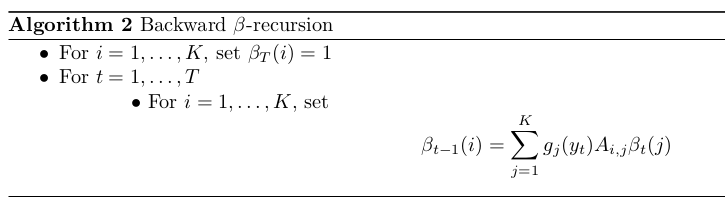
\includegraphics[scale=0.45]{images/backward_beta_recursion.jpg}
	\caption{Backward $\beta$-recursion Algorithm}
\end{figure}
\end{frame}

\begin{frame}
\frametitle{Forward-backward Smoothing IV}
\textbf{Backward and Forward Algorithm for smoothing:}

\begin{itemize}
	\item Algorithm 1 Forward $\alpha$-recursion to get $\alpha_t(x_t)=p(x_t , y_{1:t})$.
	\item Algorithm 2 Backward $\beta$-recursion to get $\beta_t(x_t)=p(y_{t+1:T} |x_t )$.
	\item Smoothing probability mass function is estimated as:
	
	$$ p(x_t | y_{1:T}) = \frac{p(x_t, y_{1:T})}{p(y_{1:T})}=\frac{\alpha_t(x_t) \beta_t(x_t)}{\sum_{x_t \in \mathcal{X}} \alpha_t(x_t) \beta_t(x_t)}$$

\end{itemize}
\vspace{0.5cm}
 \textbf{Notes:} 1) Algorithms 1 y 2 can be run independently, 2) Backward and Forward Algorithm is from order $\mathcal{O}(T\cdot|\mathcal{X}|^2)$

\end{frame}

\begin{frame}
\section{Likelihood}
\frametitle{Likelihood}

\textbf{Given:} all observations (i.e. $y_{1:T}$ known),\\
\textbf{Problem:} compute $p(y_{1:T})$ likelihood function of observations.

\vspace{0.5cm}

\textbf{Ideas:}

\begin{itemize}
	\item Notice $$p(y_{1:T} ) = \sum_{x_t \in \mathcal{X}} p(x_t , y_{1:t} ) \cdot p(y_{t+1:T} |x_t )$$
	\item This implies $$p(y_{1:T} ) = \sum_{x_t \in \mathcal{X}} \alpha_t(x_t) \beta_t(x_t) $$
	
	\item $p(y_{1:T} )$ can be estimated using algorithm 1 Forward $\alpha$-recursion and algorithm 2 Backward $\beta$-recursion.
	
\end{itemize}

\end{frame}


\begin{frame}
\frametitle{Example: Hidden Mark-frog Chains - Smoothing pmf}
\begin{center}
	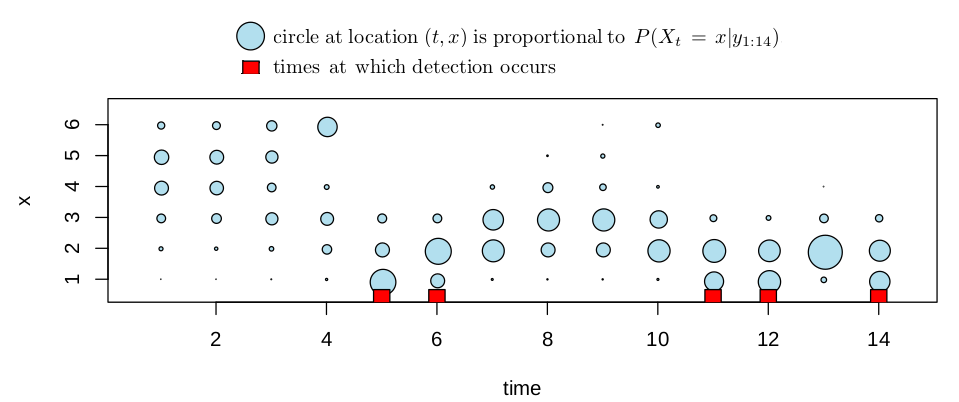
\includegraphics[width=1.01\textwidth]{images/frog_smooth.png}
\end{center}
\end{frame}

\begin{frame}
\section{Most likely state path/Decoding}
\frametitle{Most likely state path/Decoding}

\textbf{Given:} history of observations (i.e. $y_{1:T}$ known),\\
\textbf{Problem:} Find the most likely state history $x_{0:T}$.

\vspace{0.5cm}

For fixed $y_{1:T}$, solve MAP problem with \textbf{conditional distribution}:
\begin{equation*}
\hat{x}_0 = argmax_{x_{0:T}} \hspace{0.2cm} p(x_{0:T}| y_{1:T}) 
\end{equation*}
Or equivalently with \textbf{joint distribution}:
\begin{equation*}
\hat{x}_0 = argmax_{x_{0:T}} \hspace{0.2cm} p(x_{0:T}, y_{1:T})
\end{equation*}

\textbf{Note:} unfeasible if number of different state paths $|\mathcal{X}|^{T+1}$ is large from optimization point of view!!.

\end{frame}

\begin{frame}
\frametitle{Most likely state path - Viterbi algorithm}

However, we can use \textbf{Viterbi algorithm} to do MAP estimation.

\textbf{Ideas:}

\begin{itemize}
	\item Explote structure of HMM do estimations based on backward-forward or forward-backward recursions.
	\item Compute \textcolor{red}{messages} from time $t$  to $t-1$ ($m_{t-1}(x_{t-1}) \leftarrow m_{t}(x_{t})$)
	\item Use \textcolor{red}{messages} to estimate feasible points $t-1$  to $t$ ($\hat{x}_{t-1} \rightarrow \hat{x}_{t}$)	
\end{itemize}

\begin{figure}
	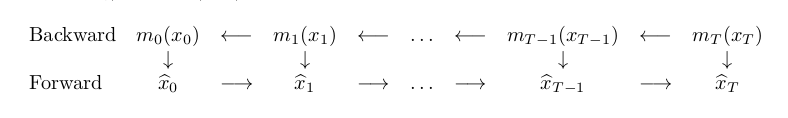
\includegraphics[scale=0.4]{images/viterbi1.jpg}
	\caption{Scheme of Vitterbi algorithm recursions}
\end{figure}

\end{frame}

\begin{frame}
\frametitle{What do you mean by \textcolor{red}{messages $m_t(x_t)$}? Part I}

Factorizing $p(x_{0:T},y_{1:T})$:
$$p(x_{0:T},y_{1:T}) = p(x_0)\prod_{t=1}^T p(x_{t}|x_{t-1}) p(y_{t}|x_{t})$$
We can split our optimization problem in different optimization problems:
$$\Rightarrow \max_{ \textcolor{red}{ x_0:x_T} } p(x_{0:T},y_{1:T}) =$$ 
$$ \max_{ \textcolor{red}{ x_0:x_{T-1}} } \left\{ \left\{ p(x_0)  \prod_{t=1}^{\textcolor{red}{T-1}} p(x_{t}|x_{t-1}) p(y_{t}|x_{t}) \right\} \max_{ \textcolor{red}{ x_{T}} } p(x_{\textcolor{red}{T}}|x_{\textcolor{red}{T-1}}) p(y_{\textcolor{red}{T}}|x_{\textcolor{red}{T}})  \right \}$$
$$=\max_{ \textcolor{red}{ x_0:x_{T-1}} } \left\{ \left\{ p(x_0)  \prod_{t=1}^{\textcolor{red}{T-1}} p(x_{t}|x_{t-1}) p(y_{t}|x_{t}) \right\} m_{\textcolor{red}{T-1}}(x_{\textcolor{red}{T-1}})  \right \}$$

\end{frame}

\begin{frame}
\frametitle{What do you mean by \textcolor{red}{messages $m_t(x_t)$}? Part II}

Continuing this process we can define a set of messages based on iterative optimization problems:
$$m_{t-1}(x_{t-1}) = \max_{  x_{t:T} }\left\{    \prod_{k=t}^{T} p(x_{k}|x_{k-1}) p(y_{k}|x_{k}) \right\} \mbox{ for } t=T-1, \ldots, 1$$
$$m_T(x_T)=1$$

\vspace{0.3cm}

This satisfies the following recursion:

$$ \textcolor{red}{m_{t-1}(x_{t-1})}  = \max_{  x_{t} } p(y_t | x_t) p(x_t | x_{t-1}) \textcolor{red}{m_t(x_t)}$$

\end{frame}

\begin{frame}
\frametitle{What do you mean by \textcolor{red}{messages $m_t(x_t)$}? Part III}
Definitions of messages is good for our problem because:
$$p(x_0) m_0(x_0) = \max_{x_{1:T}} p(x_{0:T}, y_{1:T})$$
$$\Rightarrow \hat{x_0} = arg \max_{x_0} \left(\max_{x_{1:T}} p(x_{0:T}, y_{1:T}) \right) = arg \max_{x_0} m_0(x_0) p(x_0) $$

And also

$$ \hat{x_t} = arg \max_{x_t} p( \textcolor{red}{ \hat{x}_{0:t-1}}, x_t, x_{t+1:T},y_{1:T} )$$
$$ = arg \max_{x_t} p(\textcolor{red}{\hat{x}_{t-1}}, x_t, x_{t+1:T},y_{1:T} )$$

$$ = arg \max_{x_t} \left(\textcolor{red}{m_t(x_{t})} p(y_t|x_t)  p(x_t | \hat{x}_{t-1})\right) $$

\end{frame}

\begin{frame}
\frametitle{Most likely state path - Viterbi algorithm}
\begin{figure}
	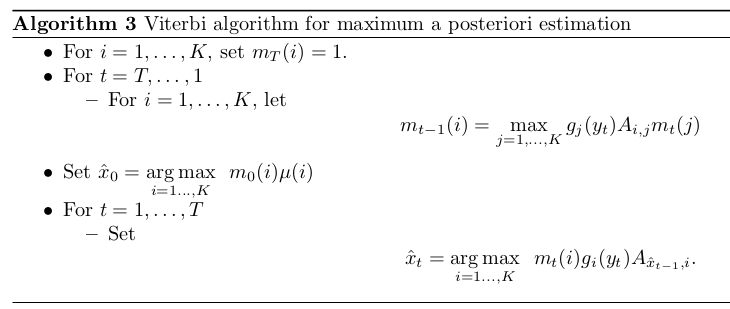
\includegraphics[scale=0.45]{images/viterbi2.jpg}
	\caption{Vitterbi algorithm}
\end{figure}

\textbf{Notes:} 1) Viterbi algorithm has order $\mathcal{O}(T |\mathcal{X}|^2)$, 2) In practice logarithms are computed to assure numerical stability.

\end{frame}

\begin{frame}
\frametitle{Example: Hidden Mark-frog Chains - MAP pmf}

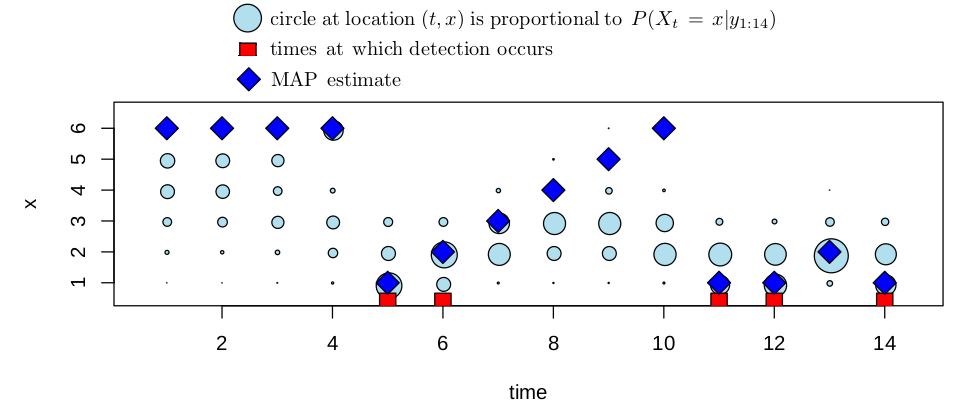
\includegraphics[width=1.01\textwidth]{images/frog_smooth_map.png}

\textbf{Note:} Image shows Smoothing pmf over time $t$ and MAP estimate
\end{frame}

\begin{frame}
\section{Continuous-state Hidden Markov Models}
\frametitle{Continuous-state Hidden Markov Models}

In many problems often hidden parameters of interest are continuous. 

\begin{figure}
	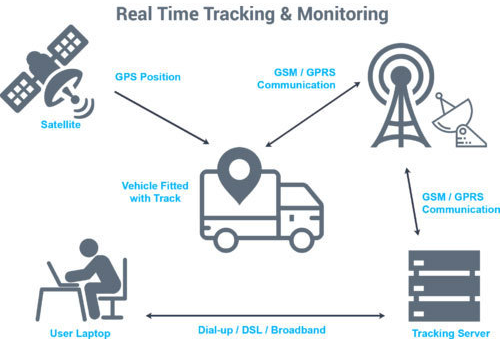
\includegraphics[scale=0.45]{gps_cut.png}
	\caption{GPS object tracking; hidden parameters: position + velocity}
\end{figure}
\end{frame}

\begin{frame}
\frametitle{Continuous-state Hidden Markov Models}
\begin{itemize}	

	\item Ideas developed for discrete case can be generalized to aboard problems with hidden continuous parameters of interest.\vspace{0.5cm}
	\item We call these \textbf{Continuous-state Hidden Markov Models} (CS-HMM), also named as state-space models or dynamical systems.\vspace{0.5cm}
	\item Let's focus on a particular subset of CS-HMM: \textbf{linear Gaussian state-space model} (LGSSM).
\end{itemize}

\end{frame}


\begin{frame}
\frametitle{Linear Gaussian state-space model (LGSSM)}

\textbf{Hidden states:} $(X_0, \ldots, X_T)$ continuous r.v. taking values in $\R^{d_x}$

\textbf{Observations:} $(Y_1, \ldots, Y_T)$ continuous r.v. taking values in $\R^{d_y}$\vspace{0.5cm}

$(X_0, \ldots, X_T, Y_1, \ldots, Y_T)$ is LGSSM if has two components such as: 

\begin{itemize}
\item \textbf{state model:} $X_{t}$ is a linear transformation of $X_{t-1}$ plus a linear combination of Gaussian noise.\vspace{0.5cm}

\item \textbf{observation model:} $Y_{t}$ is a linear transformation of $X_{t}$ plus Gaussian noise.
\end{itemize}
\end{frame}

\begin{frame}
\frametitle{Linear Gaussian state-space model (LGSSM)}
\begin{defi}[LGSSM - State model]

\begin{equation}
X_t = F_t X_{t-1} + G_t V_t \mbox{ for } t=1, \ldots, T \mbox{ State model }
\end{equation}

\end{defi}

\begin{itemize}
	\item $X_t \in  \R^{d_x}$ hidden state at time $t$,
	\item $F_t \in  \R^{d_x \times d_x}$ transition state matrix at time $t$,
	\item $G_t \in  \R^{d_x \times d_v}$ noise transfer matrix,
	\item $V_t \in  \R^{d_v}$ state noise matrix, $V_t \sim \mathcal{N}(0,Q_t)$.
\end{itemize}

\end{frame}

\begin{frame}
\frametitle{Linear Gaussian state-space model (LGSSM)}

\begin{defi}[Observation model]
	\begin{equation}
	Y_t = H_t X_{t} + W_t \mbox{ for } t=1, \ldots, T \hspace{1cm}  \mbox{ Observation model }
	\end{equation}
	
\end{defi}

\begin{itemize}
	\item $Y_t \in  \R^{d_y}$ observation at time $t$,
	\item $H_t \in  \R^{d_x \times d_x}$ observation matrix at time $t$,
	\item $W_t \in  \R^{d_v}$ observation noise, $W_t \sim \mathcal{N}(0,R_t)$.
\end{itemize}

\begin{defi}[Other conditions]
	\begin{itemize}
		\item $X_0\sim \mathcal{N}(\mu_0,\Sigma_0)$,
		\item $V_t \sim \mathcal{N}(0,Q_t), W_t \sim \mathcal{N}(0,R_t)$, for $t=1,\ldots T$,
		\item $X_0, V_1, \ldots V_T, W _1, \ldots W_T$  are independent.
	\end{itemize}
\end{defi}

\end{frame}

\begin{frame}
\frametitle{LGSSM and parametrization of joint pdf}

As in discrete case, joint pdf of hidden variables and observation can be described as:
\begin{equation}
p(X_{0:T}, Y_{1:T}) = \prod_{t=1}^T p(y_t|x_t) \cdot p(x_{t-1}|x_t)
\end{equation}

Using \textbf{LGSSM structure} and \textbf{properties of multivariate normal distributions} it can be shown that if $G_t Q_T G_T\in \R^{d_x \times d_x}$ has full rank then:

\begin{equation}
p(y_t|x_t) = \mathcal{N}(H_t x_{t}, R_t)
\end{equation}

%\begin{equation}
%p(x_t|x_{t-1}) = \mathcal{N}(x_t; H_t x_{t}, R_t)
%\end{equation}

\begin{equation}
p(x_t|x_{t-1}) = \mathcal{N}(F_t x_{t-1}, G_t Q_T G_T)
\end{equation}

\end{frame}




\begin{frame}
\frametitle{Inference in dynamic LGSSM}

Let's consider the following inference problem:

\textbf{P1:} Given \textbf{observations up to time} $t$ find $Y_1=y_1, \ldots, Y_t=y_t$, find joint pdf $p(x_t|y_{1:t})$.\vspace{0.5cm}

\textbf{P2:} Given \textbf{all observations} $Y_1=y_1, \ldots, Y_T=y_T$, find joint pdf $p(x_t|y_{1:T})$\vspace{0.5cm}

Both can be solve by \textbf{sequentially computation of means  and  covariance  matrices of conditionally distributions}: 1)  P1 is called \textbf{Kallman filter}, and in 2) P2 is named \textbf{Kallman smoother}.
\end{frame}

\begin{frame}
\frametitle{Inference LGSSM - Kallman filter}

\textbf{P1:} Determine $p(x_t|y_{1:t})$ of the hidden state $X_t$ given $t$ observations $y_{1:t}$. 

\begin{equation}
\mu_{t|t-1}:= E[X_t | Y_{1:t} = y_{1:t-1} ]
\end{equation}

\begin{equation}
\mu_{t|t}:= E[X_t | Y_{1:t} = y_{1:t} ]
\end{equation}

\begin{equation}
\Sigma_{t|t-1}:= E[(X_t -\mu_{t|t-1}) (X_t -\mu_{t|t-1})^T | Y_{1:t} = y_{1:t-1} ]
\end{equation}

\begin{equation}
\Sigma_{t|t}:= E[(X_t -\mu_{t|t}) (X_t -\mu_{t|t})^T | Y_{1:t} = y_{1:t} ]
\end{equation}

\end{frame}

\begin{frame}
\frametitle{Kallman filter ideas - Prediction}

Structure of LGSSM implies $p(x_t| y_{1:t-1})=\mathcal{N}( \mu_{t|t-1}, \Sigma_{t|t-1}  )$ and the existence of recursive rules: \vspace{0.5cm}

\textbf{Prediction} ($\mu_{t-1|t-1} \rightarrow \mu_{t|t-1} $) and ($\Sigma_{t-1|t-1} \rightarrow \Sigma_{t|t-1} $):
\begin{itemize}
	\item $\mu_{t|t-1} = F_t \mu_{t-1|t-1}$, 
	\item $\Sigma_{t|t-1} = F_t \Sigma_{t-1|t-1} F_t^T+ G_t Q_t G_t^T$
\end{itemize}

\end{frame}

\begin{frame}
\frametitle{Kallman filter ideas - Update/correction} 
Again, structure of LGSSM implies $p(x_t| y_{1:t})=\mathcal{N}( \mu_{t|t}, \Sigma_{t|t})$ and following recursion rule: \vspace{0.5cm}

\textbf{Update/correction} ($\mu_{t|t-1} \rightarrow \mu_{t|t} $) and ($\Sigma_{t|t-1} \rightarrow \Sigma_{t|t} $):
\begin{itemize}
	\item $\mu_{t|t} = \mu_{t|t-1} + K_{t} \nu_{t}$, 
	\item$\Sigma_{t|t-1} = (I-K_t H_t) \Sigma_{t-1|t-1}$
\end{itemize}

Where $\nu_t = y_t - \hat{y}_t$, $\hat{y}_t=E[Y_t|Y_{1:t-1}=y_{1:t-1}]=H_t\mu_{t|t-1}$ 

$K_t=\Sigma_{t|t-1}H^T S_t^{-1}$, $S_t=E[(Y_t - \hat{y}_t)(Y_t - \hat{y}_t)^T | Y_{1:t-1} = y_{1:t-1} ] = H_t\Sigma_{t|t-1}H_t^T +R_t$

$K_t$ is called \textbf{Kallman gain}
\end{frame}

\begin{frame}
\frametitle{Kallman filter ideas} 

\textbf{Recursive strategy of Kallman filter}

$p(x_t|y_{1:t})$ can be determined estimating parameters for $s\in \N$ of:
\begin{itemize}
\item $p(x_s| y_{1:s-1})=\mathcal{N}( \mu_{s|s-1}, \Sigma_{s|s-1})$
\item $p(x_s| y_{1:s})=\mathcal{N}( \mu_{s|s}, \Sigma_{s|s})$
\end{itemize}

as follows:

$$(\mu_0, \Sigma_0) \xrightarrow[]{\text{Predict.}} (\mu_{1|0}, \Sigma_{1|0}) \xrightarrow[]{\text{Update}} \ldots $$ 
$$\ldots \xrightarrow[]{\text{Predict.}} (\mu_{t-1|t-1}, \Sigma_{t-1|t-1})\xrightarrow[]{\text{Update}}$$ 
$$(\mu_{t|t-1}, \Sigma_{t|t-1}) \xrightarrow[]{\text{Predict.}} (\mu_{t|t}, \Sigma_{t|t}) \xrightarrow[]{\text{}} \ldots $$

\end{frame}

\begin{frame}
\frametitle{Inference LGSSM - Kallman Smoother}

 \textbf{P2:} Determine $p(x_t|y_{1:T})$ of the hidden state $X_t$ given all the observations $y_{1:T}$. 

\begin{equation}
\mu_{t|T}:= E[X_t | Y_{1:T} = y_{1:T} ]
\end{equation}

\begin{equation}
\Sigma_{t|T}:= E[(X_t -\mu_{t|T}) (X_t -\mu_{t|T})^T | Y_{1:T} = t_{1:T} ]
\end{equation}

\end{frame}


\begin{frame}
\frametitle{Kallman Smoother ideas}

Structure of LGSSM implies $p(x_t| y_{1:T})=\mathcal{N}( \mu_{t|T}, \Sigma_{t|T}  )$ and the existence of recursive rules: \vspace{0.5cm}

\textbf{Backward recursion}:
\begin{itemize}
	\item $\mu_{t|T} = \mu_{t|t} + J_t (\mu_{t+1|T} - \mu_{t+1|t})$, 
	\item $\Sigma_{t|T} = \Sigma_{t|t} + J_t (\Sigma_{t+1|T} - \Sigma_{t+1|t})J_t^T$
\end{itemize}
\vspace{0.5cm}
Where $J_t = \Sigma_{t|t} F_{t+1}^T \Sigma_{t+1|t}^{-1}$, is called \textbf{Backwards Kallman gain}.

\end{frame}

\begin{frame}

\textbf{Recursive strategy of Kallman Smoother}

$p(x_t|y_{1:T})$ can be determined estimating parameters as follows:

\begin{itemize}
	\item Compute $(\mu_{t|t}, \Sigma_{t|t})$ and $(\mu_{t+1|t}, \Sigma_{t+1|t})$ for $t,t+1 \leq T$ using Kallman filter.
	\item Use backward recursion until obtain $(\mu_{t|T}, \Sigma_{t|T})$.
\end{itemize}
\end{frame}

\begin{frame}
\section{An example for LGSSM}
\frametitle{A example for LGSSM}
Let's consider a toy example for a random walk given by:
$$X_t = X_{t-1} + V_t $$
$$Y_t = X_{t} + W_t $$

Where 

\begin{itemize}
	\item$X_{t}$: trigonometric function plus gaussian noise, for $t=1,\ldots, 50$.
	\item $X_0 = \mathcal{N}(0,1)$, $V_t \sim \mathcal{N}(0,Q)$, $W_t \sim \mathcal{N}(0,R)$, with $Q=0.02$ and $R=0.2$
\end{itemize}



\end{frame}


\begin{frame}
\frametitle{Filtering}
\begin{figure}
	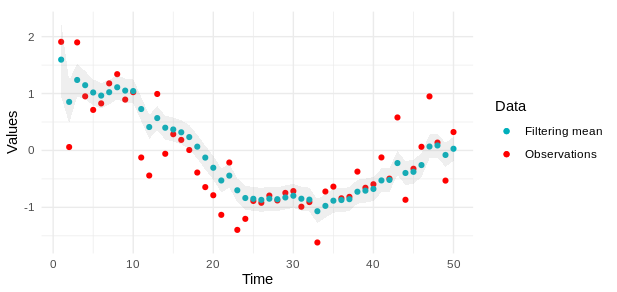
\includegraphics[scale=0.7]{filtermean_obs.png}
	\caption{Observations and filtering mean and 99\% credible intervals over time.}
\end{figure}
\end{frame}

\begin{frame}
\frametitle{Smoothing}
\begin{figure}
	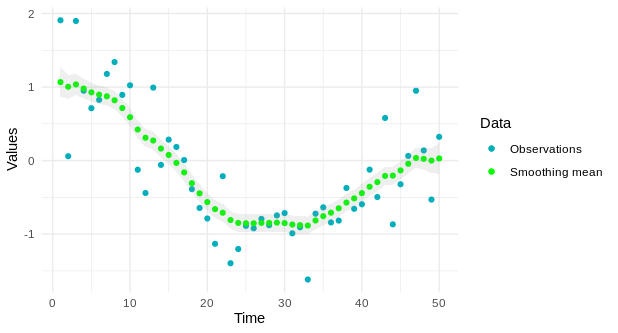
\includegraphics[scale=0.7]{smoothmean_obs.png}
	\caption{Observations and smoothing mean and 99\% credible intervals over time}
\end{figure}
\end{frame}

\begin{frame}
\section{References}
\frametitle{References}
\begin{itemize}
	\item Francois Caron, University of Oxford, Febrero 2019. Lecture notes: Hidden Markov Models. See \url{http://www.stats.ox.ac.uk/~caron/teaching/sb1b/lecturehmm.pdf}
	\item Emilio Frazzoli, Aeronautics and Astronautics (MIT), Noviembre 2010. Principes of Autonomy and Decision Making. Lecture 20: Intro to Hidden Markov Models. See \url{https://ocw.mit.edu/courses/aeronautics-and-astronautics/16-410-principles-of-autonomy-and-decision-making-fall-2010/lecture-notes/MIT16_410F10_lec20.pdf}
	\item A friendly introduction to Bayes Theorem and Hidden Markov Models. Luis Serrano, Udacity \url{https://www.youtube.com/watch?v=kqSzLo9fenk}.
\end{itemize}
	
\end{frame}

%
%\begin{frame}[fragile] % Notice the [fragile] option %
%\frametitle{Verbatim}
%\begin{example}[Putting Verbatim]
%\begin{verbatim}
%\begin{frame}
%\frametitle{Outline}
%\begin{block}
%{Why Beamer?}
%Does anybody need an introduction to Beamer?
%I don't think so.
%\end{block}
% Extra carriage return causes problem with verbatim %
%\end{frame}\end{verbatim} 
%\end{example}
%\end{frame}
 
%\begin{frame}[fragile]  % notice the fragile option, since the body
			% contains a verbatim command
%Example of the \verb|\cite| command to give a reference is below:
%Example of citation using \cite{key1} follows on.
%\end{frame}
 
% \begin{frame}
% \section{Bibliografía}
% \frametitle{Referencias}
% \footnotesize{
% \begin{thebibliography}{99}
%  \bibitem[Morita, 2010]{key1} J. Nagata, K. Morita (1989)
%  \newblock Topics On General Topology.
%  \newblock \emph{Elsevier Science Publisher B.V.} 15(6), 203 -- 243.

% \bibitem[VanMill, 2010]{key1} J. Van Mill ; M. Husek (1992)
%  \newblock Recent Progress In General Topology.
%  \newblock \emph{Elsevier Publications} p. 375.

% \bibitem[MacLane, 2010]{key1} J. S. Mac Lane(1971)
%  \newblock Categories for the working mathematician,.
%  \newblock \emph{Springer} p. 375.

%  \bibitem[Ishii, 2010]{key1} Tadashi Ishii (1969)
%  \newblock On Tychonoff Functor and $w$-Compactness.
%  \newblock \emph{Topology Appl.} 11, 175 -- 187.

%  \bibitem[Ishii, 2010]{key1} T. Hoshina; K. Morita (1980)
%  \newblock On Regular Products Of Topological Spaces.
%  \newblock \emph{Topology Appl.} 11, 47 -- 57.
% \end{thebibliography}
% }
% \end{frame}


 
% \begin{frame}
% %\section{Bibliografía}
% \frametitle{Referencias}
% \footnotesize{
% \begin{thebibliography}{99}
%  \bibitem[Porter, 2010]{key1}J. R. Porter ; R. Grant Woods  (1987)
%  \newblock Extensions and Absolutes of Hausdorff Spaces.
%  \newblock \emph{Springer-Verlag} 856.


%  \bibitem[Simon, 2010]{key1} Petr Simon (1984)
%  \newblock Completely regular modification and products.
%  \newblock \emph{Commentationes Mathematicae Universitatis Carolinae} 25(1), 121--128.



%  \bibitem[Puppier, 2010]{key1} René Puppier (1969)
%  \newblock La Completion Universelle D'un Produit D'espaces Completement Reguliers .
%  \newblock \emph{Publ. Dept. Math, Lyon} 254, 342--351.



% \end{thebibliography}
% }
% \end{frame}
% 
% End of slides
\end{document} 